
%%%%%%%%%%%%%%%%%%%%%%%%%%%%%%%%%%%%%%%%%%%%%%%%%%%%%%%%%%%%%%%%%%%%%%%%%%%%%%%%%%%%%%%%%%%%%%%%%%%%%%%%%%%%
% Author: Omar Portillo
%%%%%%%%%%%%%%%%%%%%%%%%%%%%%%%%%%%%%%%%%%%%%%%%%%%%%%%%%%%%%%%%%%%%%%%%%%%%%%%%%%%%%%%%%%%%%%%%%%%%%%%%%%%%

%Abstract: 0.5
%Intro: 2
%Bg: 2
%Approach/Architecture: 3
%Experiments/Results: 5
%Related Work: 1
%Conclusions: 0.5
%References:  1

%%%%%%%%%%%%%%%%%%%%%%%%%%%%%%%%%%%%%%%%%%%%%%%%%%%%%%%%%%%%%%%%%%%%%%%%%%%%%%%%%%%%%%%%%%%%%%%%%%%%%%%%%%%%
% Defining document class + packages to be used
%%%%%%%%%%%%%%%%%%%%%%%%%%%%%%%%%%%%%%%%%%%%%%%%%%%%%%%%%%%%%%%%%%%%%%%%%%%%%%%%%%%%%%%%%%%%%%%%%%%%%%%%%%%%

\documentclass[runningheads,a4paper]{llncs}

\usepackage{amssymb}
\setcounter{tocdepth}{3}
\usepackage{graphicx}
\usepackage{epstopdf}
\usepackage[linesnumbered,ruled,vlined]{algorithm2e}

\usepackage{url}
\newcommand{\keywords}[1]{\par\addvspace\baselineskip
\noindent\keywordname\enspace\ignorespaces#1}

%Commands needed to define the max size a float can have without been presented
% ALONE in a page.
\renewcommand\topfraction{0.85}
\renewcommand\bottomfraction{0.85}
\renewcommand\textfraction{0.1}
\renewcommand\floatpagefraction{0.85}

%Commands to redice the space before and after floats (like table,fig or alg)
\setlength\floatsep{1.25\baselineskip plus 3pt minus 2pt}
\setlength\textfloatsep{1.25\baselineskip plus 3pt minus 2pt}
\setlength\intextsep{1.25\baselineskip plus 3pt minus 2 pt}

\setlength{\belowcaptionskip}{-7.5pt}
\setlength{\abovecaptionskip}{-2.5pt}

\begin{document}

%%%%%%%%%%%%%%%%%%%%%%%%%%%%%%%%%%%%%%%%%%%%%%%%%%%%%%%%%%%%%%%%%%%%%%%%%%%%%%%%%%%%%%%%%%%%%%%%%%%%%%%%%%%%
% TITLE + AUTHORS' INFORMATION
%%%%%%%%%%%%%%%%%%%%%%%%%%%%%%%%%%%%%%%%%%%%%%%%%%%%%%%%%%%%%%%%%%%%%%%%%%%%%%%%%%%%%%%%%%%%%%%%%%%%%%%%%%%%

\mainmatter  % start of an individual contribution

% first the title is needed
\title{Towards an Automated Approach to Use Expert Systems
in Performance Testing}

% a short form should be given in case it is too long for the running head
\titlerunning{Automated Approach to Use Expert Systems
in Performance Testing}

% the name(s) of the author(s) follow(s) next
%
% NB: Chinese authors should write their first names(s) in front of
% their surnames. This ensures that the names appear correctly in
% the running heads and the author index.
%
\author{A. Omar Portillo-Dominguez\inst{1}\and Miao Wang\inst{1}\and Philip
Perry\inst{1} \and\\
John Murphy\inst{1} \and Nick Mitchell\inst{2}\and Peter F. Sweeney\inst{2}}

\authorrunning{A.O. Portillo-Dominguez et al.}
% (feature abused for this document to repeat the title also on left hand pages)

\urldef{\mailucdconnect}\path|andres.portillo-dominguez@ucdconnect.ie,|
\urldef{\mailucd}\path|{philip.perry,miao.wang,j.murphy}@ucd.ie,|
\urldef{\mailibm}\path|{nickm,pfs}@us.ibm.com|

% the affiliations are given next; don't give your e-mail address
% unless you accept that it will be published
\institute{Lero - The Irish Software Engineering Research Centre, Performance\\
Engineering Laboratory, UCD School of Computer Science and Informatics,
University College Dublin, Ireland\\
\mailucdconnect\\
\mailucd\\
%\url{http://www.ucd.ie/}
\and
IBM T.J. Watson Research Center,\\
Yorktown Heights, New York, USA\\
\mailibm}%\\
%\url{http://www.ibm.com/}

\toctitle{Lecture Notes in Computer Science}
\tocauthor{Authors' Instructions}
\maketitle

%%%%%%%%%%%%%%%%%%%%%%%%%%%%%%%%%%%%%%%%%%%%%%%%%%%%%%%%%%%%%%%%%%%%%%%%%%%%%%%%%%%%%%%%%%%%%%%%%%%%%%%%%%%%
% Abstract 
%%%%%%%%%%%%%%%%%%%%%%%%%%%%%%%%%%%%%%%%%%%%%%%%%%%%%%%%%%%%%%%%%%%%%%%%%%%%%%%%%%%%%%%%%%%%%%%%%%%%%%%%%%%%
\vspace{-15pt}
\begin{abstract}
Performance testing in highly distributed environments is a very challenging
task. Specifically, the identification of performance issues and
the diagnosis of their root causes are time-consuming and complex
activities which usually require multiple tools and heavily rely on expertise. 
To simplify the above tasks, hence increasing the productivity and reducing the
dependency on expert knowledge, many researchers have been developing tools with 
built-in expertise knowledge for non-expert users. However, variant usability
limitations exist in these tools that prevent their efficient usage in performance 
testing. To addresses these limitations, this paper presents a lightweight approach 
to automate the usage of expert tools in performance testing. In this work, we
use a tool named Whole-system Analysis Idle Time to demonstrate how our
research work solves this problem. Our validation involved two case studies using real-life
applications, assessing the proposed approach in terms of the
overhead cost and the time savings it brings to the analysis of performance
issues. The results have proven the benefits of the approach by
achieving a good decrement in the time invested in performance analysis 
while generating a low overhead in the tested system.

\vspace{-2pt}
\keywords{Performance testing, automation, performance analysis, idle-time
analysis, distributed environments, multi-tier applications}
\end{abstract}
\vspace{-22pt}
%%%%%%%%%%%%%%%%%%%%%%%%%%%%%%%%%%%%%%%%%%%%%%%%%%%%%%%%%%%%%%%%%%%%%%%%%%%%%%%%%%%%%%%%%%%%%%%%%%%%%%%%%%%%
% Introduction
%%%%%%%%%%%%%%%%%%%%%%%%%%%%%%%%%%%%%%%%%%%%%%%%%%%%%%%%%%%%%%%%%%%%%%%%%%%%%%%%%%%%%%%%%%%%%%%%%%%%%%%%%%%%
\vspace{-2pt}
\section{Introduction}
\vspace{-5pt}
It is an accepted fact in the industry that performance is a critical dimension
of quality and should be a major concern of any software project. This is
especially true at enterprise-level, where performance plays a central role in
usability. However it is not uncommon that performance issues occur and
materialize into serious problems in a significant percentage of projects (i.e.
outages on production environments or even cancellation of projects). For
example, a 2007 survey applied to information technology executives
\cite{Compuware1} reported that 50\% of them had faced performance problems in at 
least 20\% of their deployed applications.

This situation is partially explained by the pervasive nature of
performance, which makes it hard to assess because performance is practically
influenced by every aspect of the design, code, and execution environment
of an application. Latest trends in the information technology world (such as
Service Oriented Architecture and Cloud Computing) have also augmented the
complexity of applications further complicating activities related to
performance. Under these conditions, it is not surprising that doing performance
testing is complex and time-consuming. A special challenge, documented by
multiple authors \cite{Woodside2007,trevor1,Angelopoulos2012}, is that current
performance tools heavily rely on expert knowledge to understand their output.
It is also common that multiple sources are required to diagnose
performance problems, especially in highly distributed environments. For
instance in Java: thread dumps, garbage collection logs, heap dumps, CPU
utilization and JVM memory usage, are a few examples of the information that a
tester could need to understand the performance of an application. This
situation increases the expertise required to do performance analysis, which is
usually held by only a small number of testers within an organization. It
could potentially lead to bottlenecks where some activities can only be done by
experts, impacting the productivity of large testing teams.

To simplify the performance analysis and diagnosis tasks, hence increasing the
productivity and reducing the dependency on expert knowledge, many researchers
have been developing tools with built-in expertise knowledge for non-expert
users \cite{Altman2010,pat7,Angelopoulos2012}. However, various limitations
exist in these tools that prevent their efficient usage in performance testing.
The data collection process usually needs to be controlled manually, which in a
highly distributed environment (composed of multiple nodes to monitor and
coordinate simultaneously) is very time-consuming and error-prone, specially if
the data needs to be processed periodically during the test execution to have an
incremental view of the results. The same situation occurs with the outputs,
where a tester commonly needs to review multiple reports, one for each monitored
node per data processing cycle.

Even though these limitations might be manageable in small testing environments,
they prevent an effective usage of an expert system in bigger testing
environments. For example, consider an application composed of 10 nodes, a
24-hour test run and an interval of 1 hour to get incremental results. A tester
would need to manually coordinate to stop the data collections, generate the
outputs of the expert system and then start the data collections again. These
steps conducted for the 10 nodes in cycles of 1 hour, which throws a total of
240 cycles. Additionally, these steps would need to be carried out as fast as
possible to minimize the time gaps between the end of a cycle and the start of
the next. Lastly, the tester would have to review the 10 different reports she
would get every hour and compare them with the previous ones to evaluate if
there are any performance issues. As it can be inferred from this example, the
costs of using an expert system in a highly distributed environment would
outweigh its benefits. As an alternative, testers may chose to focus the analysis on a single node, assuming it is representative of the whole system. However this
assumption generates the risk of potential overlooking other issues in the
tested application.

In addition to the previous challenges, the overhead generated by any technique
should be low to minimize the impacts it has in the tested environment (i.e.
inaccurate results or abnormal behaviors), otherwise the technique would not be
suitable for performance testing. For example,
instrumentation\footnote{http://msdn.microsoft.com/en-us/library/aa983649(VS.71).aspx}
is currently a common approach used in performance analysis to gather input data
\cite{Yang1,Hangal1,Csallner1,Chen2}. However, it has the downsize of obscuring
the performance of the instrumented applications, hence compromising the results of 
performance testing. Similarly, if a tool requires heavy human effort to be
used, this might limit the applicability of that tool. On the contrary, automation 
could play a key role to encourage the adoption of a technique. As documented by
the authors in \cite{Shahamiri1}, this strategy has proven successful in
performance testing activities.

Finally, to ensure that our research work is helpful for solving real-life
problems in the software industry, we have been working with our industrial
partner, the IBM System Verification Test (SVT), to understand the challenges
that they experience in their day-to-day testing activities. The received
feedback confirms that there is a real need to simplify the usage of expert
tools so that testers can carry out analysis tasks in less time.

This paper proposes a lightweight automation approach that addresses the common
usage limitations of an expert system in performance testing. Furthermore,
during our research development work we have successfully applied our approach to 
the IBM Whole-system Analysis of Idle Time tool
(WAIT)\footnote{http://wait.ibm.com}. This publicly available tool is a
lightweight expert system that helps to identify the main performance inhibitors
that exist on Java systems. Our work was validated through two case studies 
using real-world applications. The first case study concentrated in
evaluating the overhead introduced by our approach. The second
assessed the productivity gains that the approach brings to the
performance testing process. The current results have provided evidence about
the benefits of this approach: It drastically reduced the effort required by a
tester to use and analyze the outputs of the selected expert tool (WAIT). This
usage simplification translated into a quicker identification of performance issues, including the pinpointing of the
responsible classes and methods. Also the introduced overhead was low
(between 0\% to 3\% when using a common industry \emph{Sampling Interval}).

The main contributions of this paper are: 
%\\\\

1. A novel lightweight approach to automate the usage of expert systems in
performance testing.

2. A practical validation of the approach consisting of an implementation
around the WAIT tool and two case studies using real-life applications.

3. Analysis of the overhead the approach has in the monitored environment.
\\\\
The rest of this paper is structured as follows: Section \ref{Background}
discusses the background. Section \ref{ProposedApproach} explains the proposed approach, while Section
\ref{ExperimentalEvaluation} explores the experimental evaluation and results.
Section \ref{RelatedWork} shows the related work. Finally Section
\ref{Conclusions} presents the conclusions and future work.


%%%%%%%%%%%%%%%%%%%%%%%%%%%%%%%%%%%%%%%%%%%%%%%%%%%%%%%%%%%%%%%%%%%%%%%%%%%%%%%%%%%%%%%%%%%%%%%%%%%%%%%%%%%%
% Background
%%%%%%%%%%%%%%%%%%%%%%%%%%%%%%%%%%%%%%%%%%%%%%%%%%%%%%%%%%%%%%%%%%%%%%%%%%%%%%%%%%%%%%%%%%%%%%%%%%%%%%%%%%%%
\vspace{-5pt}
\section{Background}
\label{Background}
\vspace{-5pt}
\emph{Idle-time analysis} is a methodology that pursues to explain the root
causes that lead to under-utilized resources. This approach, proposed in
\cite{Altman2010}, is based on the observed behavior that performance problems in multi-tier
applications usually manifest as idle time indicating a lack of motion.
WAIT is an expert system that implements the idle-time analysis and identifies
the main performance inhibitors that exist on a system. Moreover it has proven successful in simplifying the detection of performance issues and their root causes in Java
systems \cite{Altman2010,Wu1}.

WAIT is based on non-intrusive sampling mechanisms available at
Operating System level (i.e. ``ps'' command in a Unix environment) and the Java
Virtual Machine (JVM), in the form of \emph{Javacores}
\footnote{http://www-01.ibm.com/support/docview.wss?uid=swg27017906\&aid=1}
(diagnostic feature to get a quick snapshot of the JVM state, offering
information such as threads, locks and memory). The fact that WAIT uses standard
data sources makes it non-disruptive, as no special flags or instrumentation are
required to use it. Furthermore WAIT requires infrequent samples to perform its
diagnosis, so it also has low overhead.

From a usability perspective, WAIT is simple: A user only needs to
collect as much data as desired, upload it to a public web page and obtain a
report with the findings. This process can be repeated multiple times to monitor a
system through time. Internally, WAIT uses an engine built on top of a set of 
expert rules that perform the analysis. \figurename ~\ref{fig_WAITReport} shows an
example of a WAIT Report. The top area summarizes the usage of resources (i.e.
CPU, thread pools and Java Heap) and the number and type of threads per sample. 
The bottom section shows all the performance inhibitors that have been identified, ranked
by frequency and impact. Moreover each category of problem is indicated with a
different color. For example, in \figurename ~\ref{fig_WAITReport} the top issue
appeared in 53\% of the samples and affected 7.6 threads on average. The
affected resource was the network (highlighted in yellow) and was caused by
database readings.

\begin{figure}[!h]
\centering
\includegraphics[totalheight=.3\textheight,width=1.0\textwidth]{bigExampleReportConsolidated}
\caption{Example of WAIT Report}
\label{fig_WAITReport}
\end{figure}

Given its strengths, WAIT is a promising candidate to reduce the expert
knowledge and time required to do performance analysis. However, it has
some usability limitations that exemplify the current challenges to effectively
use an expert system in the performance testing domain: The effort required to
do manual data collection to feed WAIT and the number of WAIT reports a tester
would need to review are practically lineal with respect of the number of
application nodes and the frequency with which the data is
refreshed. This makes WAIT a good candidate to apply our proposed approach.

%%%%%%%%%%%%%%%%%%%%%%%%%%%%%%%%%%%%%%%%%%%%%%%%%%%%%%%%%%%%%%%%%%%%%%%%%%%%%%%%%%%%%%%%%%%%%%%%%%%%%%%%%%%%
% Proposed Approach
%%%%%%%%%%%%%%%%%%%%%%%%%%%%%%%%%%%%%%%%%%%%%%%%%%%%%%%%%%%%%%%%%%%%%%%%%%%%%%%%%%%%%%%%%%%%%%%%%%%%%%%%%%%%
\vspace{-5pt}
\section{Proposed Approach and Architecture}
\label{ProposedApproach}
\vspace{-5pt}

%This section presents the proposed approach and the architecture that supports
%it.

\subsection{Proposed Approach}
\vspace{-5pt}
The objective of this work was to address the common usability limitations of
expert systems (ES) to be applied effectively in performance testing. To achieve
this goal, our approach proposes the automation of the manual processes involved
in the usage of an expert system. This approach will execute jointly to the
performance test, periodically collecting the required samples, then getting
them incrementally processed by the expert system to get a consolidated output.

The detailed approach is depicted in the \figurename
~\ref{fig_ApproachDiagram}. In order to start, some inputs are
required: The list of nodes to be monitored; a \emph{Sampling Interval} to
control how often the samples will be collected; a \emph{Time Threshold} to
define the maximum time between data uploads; a \emph{Hard Disk Threshold} to
define the maximum storage quota for collected data (to prevent its uncontrolled
growth); and a \emph{Backup} flag to indicate if the collected data should be
backed up before any cleaning occurs.

\begin{figure}[!h]
\centering
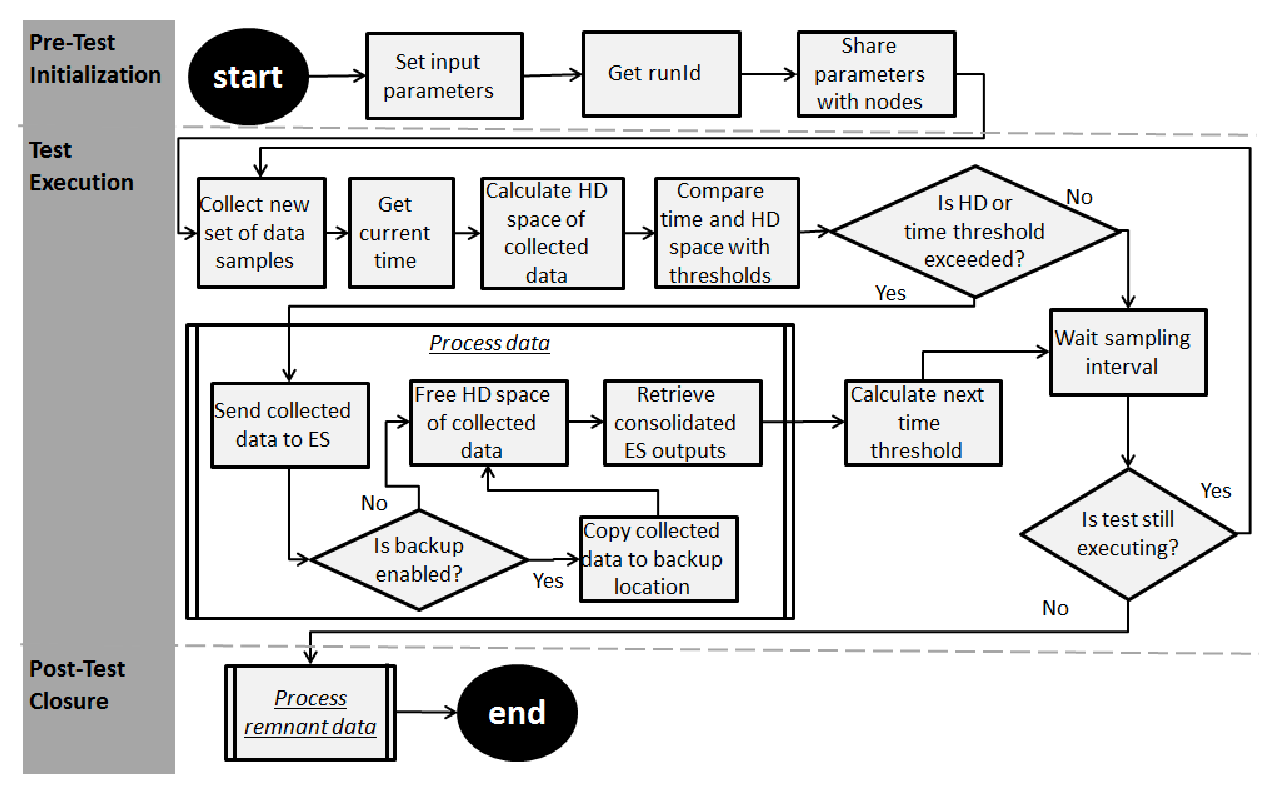
\includegraphics[width=1.0\textwidth]{ApproachDiagram}
\caption{Process Flow - Automation approach}
\label{fig_ApproachDiagram}
\end{figure}

The process starts by initializing the configured parameters. Then it gets
a new \emph{RunId}, value which will uniquely identify the test run and its reports.
This value is propagated to all the nodes. On each node, the \emph{Hard Disk
Usage} and  the \emph{Next Time Threshold} are initialized. Then each node
starts in parallel the following loop until the performance test finishes: A new
set of data samples is collected. After the collection finishes, it is assessed if any of
the two thresholds has been reached (either the \emph{Hard Disk Usage} has
exceeded the \emph{Hard Disk Threshold} or the \emph{Next Time Threshold} has
been reached). If any of these conditions has occurred, a new upload round
occurs where the data is sent to the expert system (labeling the data with the
\emph{RunId} so that information from different nodes can be identified as part
of the same test run). If a \emph{Backup} was enabled, the data is copied
to the backup destination before it is deleted to free space and
keep the HD usage below the threshold. Then updated outputs from the
expert system are retrieved and the \emph{Next Time Threshold} is calculated. Finally,
the logic awaits the \emph{Sampling Interval} before a new iteration
starts.

Once the performance test finishes, any remnant collected data is sent (and
backed up if configured) so that this information is also processed by the
expert system. Lastly this data is also cleared and the final consolidated
outputs of the expert system are obtained.

\vspace{-5pt}
\subsection{Architecture}
\vspace{-5pt}
The approach is complemented with the architecture
presented in \figurename ~\ref{fig_Arch}. It is composed of two main components:
The \emph{Control Agent} is responsible of interacting with the Load
Testing tool to know when the performance test starts and ends. It is also
responsible of getting the runId and propagate it to all the nodes. The second
component is the \emph{Node Agent} which is responsible of the collection,
upload, backup and cleanup steps in each application node. 

%\vspace{-5pt}
\begin{figure}[!h]
\centering
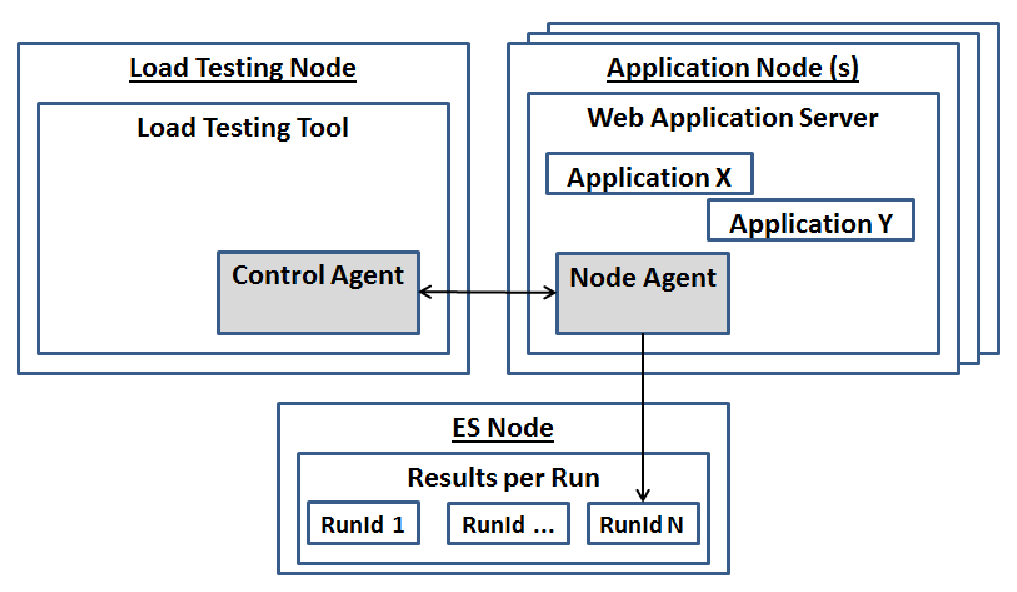
\includegraphics[totalheight=.22\textheight,width=0.8\textwidth]{architecture_dwait}
\caption{High-level architecture of automated approach}
\label{fig_Arch}
\end{figure}
%\vspace{-5pt}

These components communicate through commands, following the \emph{Command}
Design Pattern\footnote{http://www.oodesign.com/command-pattern.html}. Here the
\emph{Control Agent} invokes the start and stop commands based on the
changes of status in the Load Testing tool, while the \emph{Node Agent}
implements the logic in charge of executing each concrete command. This logic
includes sending back the result of the performed operation to the \emph{Control
Agent}.

An example of the distinct interactions that occur between these
components is depicted in \figurename ~\ref{fig_SeqDiagram}. Once a tester has
started a performance test (step 1), the \emph{Control Agent} propagates the
action to each of the nodes (steps 2 to 4). Then each \emph{Node Agent} performs
its periodic data collections (steps 5 to 9) until any of the thresholds is
satisfied and the data is sent to the ES (steps 10 and 11). These processes
continue iteratively until the test ends. At that moment, the \emph{Control
Agent} propagates the stop action to all \emph{Node Agents} (steps 21,22 and
24). At any time during the test execution, the tester might choose to review
the intermediate results obtained from the expert system (steps 12 to 14) until
getting the final results (steps 25 to 27). Moreover, the tester only needs to
interact with the Load Testing tool during the whole test execution.

\vspace{-5pt}
\begin{figure}[!h]
\centering
\includegraphics[width=1.0\textwidth]{SequenceDiagram}
\caption{Sequence diagram of the automated approach}
\label{fig_SeqDiagram}
\end{figure}
\vspace{-5pt}

%%%%%%%%%%%%%%%%%%%%%%%%%%%%%%%%%%%%%%%%%%%%%%%%%%%%%%%%%%%%%%%%%%%%%%%%%%%%%%%%%%%%%%%%%%%%%%%%%%%%%%%%%%%%
% Experimental Setup / Experiments
%%%%%%%%%%%%%%%%%%%%%%%%%%%%%%%%%%%%%%%%%%%%%%%%%%%%%%%%%%%%%%%%%%%%%%%%%%%%%%%%%%%%%%%%%%%%%%%%%%%%%%%%%%%%
\vspace{5pt}
\section{Experimental Evaluation}
\label{ExperimentalEvaluation}
%\vspace{-5pt}

%In this section the developed prototype and the experimental setup are
%presented. Then the experiments are described and their results discussed.

\vspace{-5pt}
\subsection{Prototype}
\vspace{-5pt}
Based on the proposed approach, a prototype has been developed
in conjunction with our industrial partner IBM. The \emph{Control Agent} was
implemented as an Eclipse Plugin for the Rational Performance Tester (RPT)
\footnote{http://www-03.ibm.com/software/products/us/en/performance}, which is a
load testing tool commonly used in the industry; the \emph{Node Agent} was
implemented as a Java Web Application, and WAIT was the selected expert system
due to its analysis capabilities to diagnose performance issues and their root
causes.

Once the agents are installed in the environment, WAIT can be configured as
any other resource in RPT as shown in \figurename ~\ref{fig_config}. Similarly, during a
performance test WAIT can be monitored as any other resource in the
\emph{Performance Report} of RPT under the \emph{Resource View} as depicted in
\figurename ~\ref{fig_mon}. Finally, the consolidated WAIT report is also
accessible within RPT, so a tester does not need to leave RPT during the whole
performance test. This is shown in \figurename ~\ref{fig_report}.

%--------------------------------------------------
\vspace{-5pt}
\begin{figure*}
\centering
\begin{minipage}[b]{.50\textwidth}

\centering
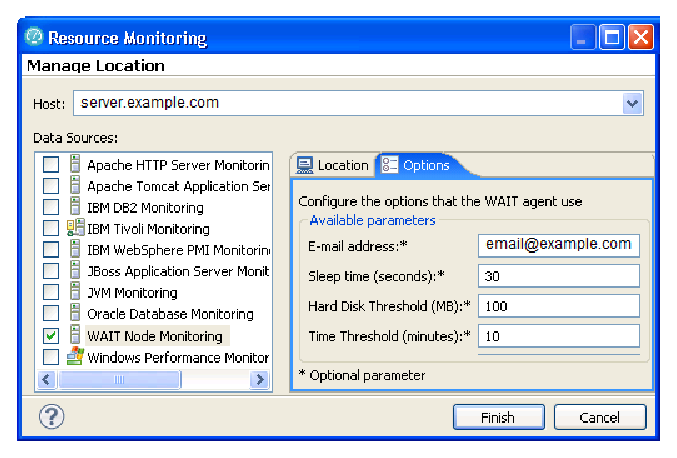
\includegraphics[totalheight=.27\textheight,width=1.0\textwidth]{WAIT-config}
\caption{WAIT configuration in RPT}
\label{fig_config}

\end{minipage}\qquad
\begin{minipage}[b]{.44\textwidth}

\centering
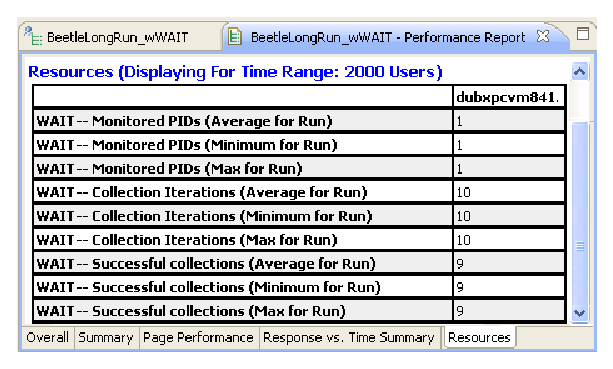
\includegraphics[totalheight=.27\textheight,width=1.0\textwidth]{WAIT-monitoring}
\caption{WAIT monitored in RPT}
\label{fig_mon}

\end{minipage}
\end{figure*}
\vspace{-5pt}

%--------------------------------------------------

\begin{figure}[!h]
\centering
\includegraphics[totalheight=.35\textheight,width=1.0\textwidth]{WAIT-report}
\caption{WAIT Report accessible in RPT}
\label{fig_report}
\end{figure}

\vspace{-5pt}
\subsection{Experimental Set-up}
\vspace{-5pt}
Two experiments were performed. The first one aimed to evaluate if the overhead
introduced by the proposed approach was low so that it does not compromise the
results of a performance test. Meanwhile, the second one pursued to
assess the productivity benefits that a tester can gain by using the proposed
approach.

Additionally two environment configurations were used. They are shown in
\figurename ~\ref{fig_env}. One was composed of a RPT node, one application node
and a \emph{WAIT Server} node; the other was composed of a RPT node, a load
balancer node, two application nodes and a \emph{WAIT Server} node. All
connected by a 10-GBit LAN.

\begin{figure}[!h]
\centering
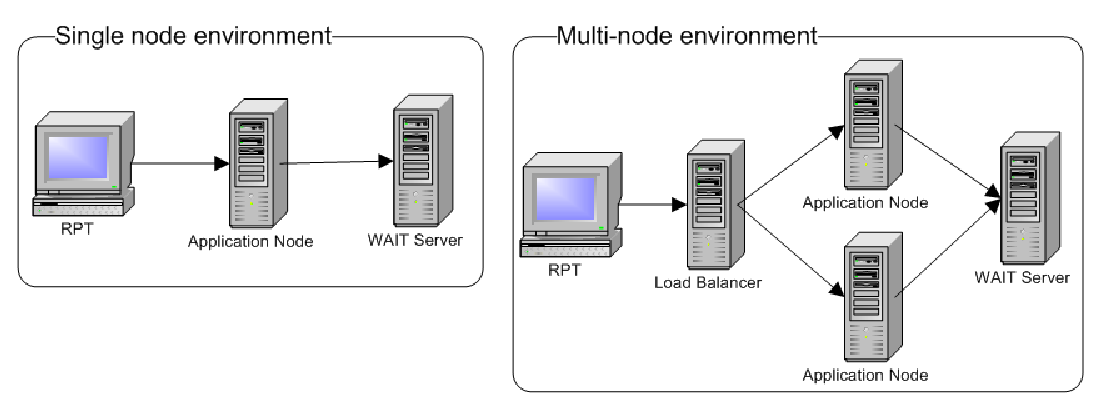
\includegraphics[totalheight=.15\textheight,width=0.9\textwidth]{Environments}
\caption{Environment Configurations}
\label{fig_env}
\end{figure}

The RPT node ran over Windows XP with an Intel Xeon CPU at
2.67 Ghz and 3GB of RAM using RPT 8.2.1.3. The \emph{WAIT Server} was run over
Red Hat Enterprise Linux Server 5.9, with an Intel Xeon CPU at 2.66 GHz and 2GB of
RAM using Apache Web Server 2.2.3. Each application node was a 64-bit Windows
Server 2008, with an Intel Xeon E7-8860 CPU at 2.26 GHz and 4GB of RAM
running Java 1.6.0 IBM J9 VM (build 2.6). Finally, the load balancer node had
the same characteristics of the \emph{WAIT Server} node. 

\vspace{-5pt}
\subsection{Experiment \#1: Overhead Evaluation}
\vspace{-2pt}

Its objective was to validate that the proposed approach had low overhead and
involved the assessment of four metrics: Throughput (hits per second), response
time (milliseconds), CPU (\%) and memory (MB) utilization. All metrics were
collected through RPT. Furthermore, two real-world applications were used:
iBatis JPetStore 4.0 \footnote{http://sourceforge.net/projects/ibatisjpetstore/}
which is an upgraded version of Sun's Pet Store, an e-commerce shopping cart. It
ran over an Apache Tomcat 6.0.35. 
% Application Server
The other application was IBM WebSphere Portal 
%Server 
8.0.1 \footnote{http://www-03.ibm.com/software/products/us/en/portalserver},
a leader solution in the enterprise portal market.  
%\cite{Gartner2008}
It ran over an IBM WebSphere Application Server 8.0.0.5.

Firstly, the overhead was measured in a single-node environment using three
combinations of WAIT: The applications alone to get a baseline; the applications
with manual WAIT data collection; and the applications with an automated WAIT.
For each combination using WAIT, the \emph{Sampling Interval} was configured
to 480 seconds (suggested by IBM SVT) and 30 seconds (minimum value recommended for
WAIT). The remaining test configuration was suggested by IBM SVT to
reflect real-world conditions: A workload of 2,000 concurrent users; a duration
of 1 hour; a \emph{Hard Disk Threshold} of 100MB; and a \emph{Time Threshold} of
10 minutes. Finally, each combination was repeated three times.

For JPetStore, each test run produced around 500,000 transactions. The results
presented in \tablename ~\ref{PetStore1} showed that using WAIT with a
\emph{Sampling Interval} of 480 seconds had practically no impact in terms of
response time and throughput. Furthermore the difference in resource consumption
between the different modalities of WAIT was around 1\%.  This difference was
mostly related to the presence of the \emph{Node Agent} because the uploaded
data was very small in this case (around 200KB every 10 minutes). When a
\emph{Sampling Interval} of 30 seconds was used, the impacts in response time
and throughput appeared. Considering the throughput was similar between the WAIT
modalities, the impact was caused by the \emph{Javacore} generation (only step
shared between the modalities). In average, the generation of a \emph{Javacore}
took around 1 second. Even though this cost was insignificant in the higher
\emph{Sampling Interval}, with 30 seconds the impact was visible. On the
contrary, the difference in response times (2.8\%, around 53 milliseconds) was
caused by the upload and backup processes (around 4MB of data every 10 minutes),
as the cost of the \emph{Node Agent} presence had been previously measured. In
terms of resource consumption, the differences between the WAIT modalities
remained within 1\%.

\begin{table}[!h]
\caption{JPetStore - Overhead Results}
\label{PetStore1}
\centering
\begin{tabular}{p{0.2\textwidth}|p{0.16\textwidth}|p{0.16\textwidth}|p{0.15\textwidth}|p{0.13\textwidth}|p{0.16\textwidth}}
\hline
\bfseries WAIT Modality & \bfseries Avg Response Time (ms)& \bfseries Max
Response Time (ms)& \bfseries Avg Throughput (hps)& \bfseries Avg CPU Usage
(\%) & \bfseries Avg Memory Usage (MB)\\
\hline
None (\emph{Baseline}) 	& 1889.6	& 44704.0	& 158.8 	& 36.9 		& 1429\\
Manual, 480s 			& 0.0\% 	& 0.0\%		& 0.0\%		& 1.1\% 	& 3.0\%\\
Automated, 480s 		& 0.0\%		& 0.0\%		& 0.0\% 	& 2.0\% 	& 3.7\%\\
Manual, 30s 			& 1.6\%		& 0.4\%		& -4.0\% 	& 1.47\% 	& 4.1\%\\
Automated, 30s 			& 4.4\%		& 0.5\%		& -3.1\% 	& 2.53\% 	& 4.4\%\\
%\hline
%Automated, 480s (2 nodes)& 0.5\%	& 0.2\%		& -1.4\% 	& 0.85\% 	& 2.3\%\\
\hline
\end{tabular}
\end{table}

For Portal, each test run produced around 400,000 transactions. Even though the
results presented in \tablename ~\ref{Portal1} showed similar trends in terms of
having lower overheads using the \emph{Sampling Interval} of 480 seconds, a few
key differences were identified: First, the impacts in response time and
throughput were visible since the \emph{Sampling Interval} of 480 seconds.
Besides, the differences between \emph{Sampling Intervals} were bigger. As the
experiment conditions were the same, it was initially assumed that these differences 
were related to the dissimilar functionality of the tested applications. This was confirmed 
after analyzing the \emph{Javacores} generated by Portal, which allowed to
quantify the differences in behavior of Portal: The average size of a \emph{Javacore} was
5.5MB (450\% bigger than JPetStore's), its average generation time was 2 sec
(100\% bigger than JPetStore's), with a maximum generation time of 3 sec (100\%
bigger than JPetStore's).

\begin{table}[!h]
\caption{Portal - Overhead Results}
\label{Portal1}
\centering
\begin{tabular}{p{0.2\textwidth}|p{0.16\textwidth}|p{0.16\textwidth}|p{0.15\textwidth}|p{0.13\textwidth}|p{0.16\textwidth}}
\hline
\bfseries WAIT Modality & \bfseries Avg Response Time (ms)& \bfseries Max
Response Time (ms)& \bfseries Avg Throughput (hps)& \bfseries Avg CPU Usage
(\%) & \bfseries Avg Memory Usage (MB)\\
\hline
None (\emph{Baseline}) 	& 4704.75	& 40435.50	& 98.05 	& 76.73 	& 3171.20\\
Manual, 480s 			& 0.7\% 	& 0.6\%		& -0.1\%	& 1.13\% 	& 2.2\%\\
Automated, 480s 		& 3.4\%		& 1.0\%		& -2.8\% 	& 0.63\% 	& 4.1\%\\
Manual, 30s 			& 14.9\%	& 5.4\%		& -5.7\% 	& 2.97\% 	& 5.3\%\\
Automated, 30s 			& 16.8\%	& 9.1\%		& -5.6\% 	& 2.23\% 	& 6.0\%\\
\hline
\end{tabular}
\end{table}

Due to the small differences among the runs and the variations (presumable
environmental) that were experienced during the experiments, a Paired t-Test
\footnote{http://www.aspfree.com/c/a/braindump/comparing-data-sets-using-statistical-analysis-in-excel/}
was done (using a significant level of p\textless0.1) to evaluate if the
differences in response time and throughput were statistically significant. 
This analysis indicated that 
%The results presented in \tablename ~\ref{tTest1} showed that 
for JPetStore the only significant differences existed in the average response
time and the average throughput (of the automated WAIT) when using a
\emph{Sampling Interval} of 30 seconds. Similar results were obtained from Portal. This analysis reinforced the
conclusion that the overhead was low and the observation that the
\emph{Sampling Interval} of 480 seconds was preferable.

%\begin{table}[!h]
%\caption{Paired t-Test Results}
%\label{tTest1}
%\centering
%\begin{tabular}{p{0.2\textwidth}|p{0.2\textwidth}|p{0.2\textwidth}|p{0.2\textwidth}|p{0.2\textwidth}}
%\hline
%\bfseries Application & \bfseries WAIT Modality & \bfseries Avg Response Time
%(ms)& \bfseries Max Response Time (ms)& \bfseries Avg Throughput (hps)\\
%\hline
%JPetStore & 	Manual, 480s 			& 0.470 & 0.143	& 0.206\\
%JPetStore & 	Automated, 480s 		& 0.342	& 0.297	& 0.472\\
%JPetStore & 	Manual, 30s 			& 0.089	& 0.241	& 0.154\\
%JPetStore & 	Automated, 30s 			& 0.019	& 0.334	& 0.078\\
%\hline
%Portal 	& 	Manual, 480s 			& 0.140 & 0.263	& 0.496\\
%Portal 	& 	Automated, 480s 		& 0.040	& 0.189	& 0.131\\
%Portal 	& 	Manual, 30s 			& 0.001	& 0.158	& 0.167\\
%Portal 	& 	Automated, 30s 			& 0.013	& 0.105	& 0.072\\
%\hline
%\end{tabular}
%\end{table}

A second test was done to validate that the overhead remained low in a
multi-node environment over a longer test run. This test used JPetStore and the
automated WAIT with a \emph{Sampling Interval} of 480 seconds. The rest of the
set-up was identical to the previous tests except the workload which was doubled
to compensate the additional application node and the test duration which was
increased to 24 hours. Even though the results were slightly different than the
single-node run, they proved that the solution was reliable, as using the
automated approach had minimal impact in terms of response time (0.5\% in the
average and 0.2\% in the max) and throughput (1.4\%). Moreover the consumption
of resources behaved similar to the single-node test (an increment of 0.85\% in
CPU and 2.3\% in Memory). A paired t-Test also indicated
that the differences in response time and throughput between the runs were
not significant.

%The performed paired t-Test also indicated
%that the differences in response time and throughput between the test runs were
%not statistically significant.

In conclusion, the results of this experiment proved that the
overhead caused by the automated approach was low. Therefore the results of a
performance test are not compromised. Due to the impact that the \emph{Sampling
Interval} and the application behavior could have in the overhead, it is important to 
consider these factors in the configuration. In our case, a \emph{Sampling
Interval} of 480 seconds proved efficient in terms of overhead for the two tested applications using WAIT.

\vspace{-5pt}
\subsection{Experiment \#2: Assessment of productivity benefits}
\vspace{-2pt}

Here the objective was to assess the benefits our approach brings to a
performance tester. First, the source code of JPetStore was modified and three
common performance issues were injected: A lock contention bug, composed of a
very heavy calculation within a synchronized block of code; a I/O latency bug, 
composed of a very expensive file reading method; and a deadlock bug, compose
of an implementation of the classic ``friends bowing'' deadlock
example\footnote{http://docs.oracle.com/javase/tutorial/essential/concurrency/deadlock.html}.
Then an automated WAIT monitored the application to assess how well
it was able to identify the injected bugs and estimate the corresponding time
savings in performance analysis. All set-up parameters were identical to
the multi-node test previously described except the duration which
was one hour. Due to space constraints, only the most relevant sections
of the WAIT reports are presented.

Surprisingly the 1st ranked issue was none of the injected bugs but a method
named ``McastServiceImpl.receive'' which appeared in practically all the
samples. Further analysis determined this method call was benign and related
to the clustering functionality of Tomcat. The 2nd ranked issue was the lock
contention. A relevant point to highlight is that both issues were detected
since the early versions of the report. Their high frequency (above
96\% of the samples) could have led a tester to pass this
information to the development team so that the diagnosis could start far ahead
of the test completion. The final report reinforced the presence of these issues 
by offering similar rankings. \figurename ~\ref{fig_run1_bugs12}.a shows the
results of the early report, while ~\ref{fig_run1_bugs12}.b shows the results of the final report.

\begin{figure}[!h]
\centering
\includegraphics[totalheight=.25\textheight,width=1\textwidth]{big_issues12_run1_earlyVsFinalReport}
\caption{Top detected performance issues in modified JPetStore application}
\label{fig_run1_bugs12}
\end{figure}

\begin{figure}[!h]
\centering
\includegraphics[totalheight=.25\textheight,width=1\textwidth]{lockContentionIssue_WAITvsEclipse_Highlighted}
\caption{Lock contention issue in the WAIT report and the actual source code}
\label{fig_issue2_vs_code}
\end{figure}

After identifying an issue, a tester can see more details, including the type of
problem, involved class, method and method line. \figurename
~\ref{fig_issue2_vs_code} shows the information of our Lock Contention bug,
which was located in the class LockContentionBug, the method generateBug and the
line 20. When comparing this information with the actual code, one can see that
is precisely the line where the bug was injected (taking a class lock before
doing a very CPU intensive logic). In 3rd place the report showed a symptom of
the lock contention issue, suggesting this was a major problem (the issues were correlated 
by comparing their detailed information, which pinpointed to the same class and
method). Finally, the I/O latency bug was identified in 4th place. \figurename
~\ref{fig_issues34} shows the details of these issues.

\begin{figure}[!h]
\centering
\includegraphics[totalheight=.25\textheight,width=1\textwidth]{big_issue3and4_run1_finalReportDetailsMerge}
\caption{Details of issues ranked 3rd and 4th}
\label{fig_issues34}
\end{figure}

The deadlock issue did not appear in this test run, somehow prevented by the
lock contention bug which had a bigger impact that planned. As in any regular
test phase, the identified bugs were ``fixed'' and a new run was done to review
if any remaining performance issues existed. Not surprisingly, the deadlock bug
appeared. \figurename ~\ref{fig_dlissue_vs_code} shows the information of our
Deadlock bug, which was located in the line 30 of the DeadLockBug class. This is
precisely the line where the bug was injected (as the deadlock occurs when the
friends bow back to each other).
\vspace{-5pt}
\begin{figure}[!h]
\centering
\includegraphics[totalheight=.23\textheight,width=1\textwidth]{deadlockIssue_DetailsVsEclipse_Highlight}
\caption{Deadlock issue in the WAIT report and the actual source code}
\label{fig_dlissue_vs_code}
\end{figure}
\vspace{-5pt}

As all injected bugs were identified, including the involved classes and
methods, this experiment was considered successful. In terms of time, two main
savings were documented. First, the automated approach practically reduced the
effort of using WAIT to zero. After a one-time installation which took no more
than 15 minutes for all nodes, the only additional effort required to use the
automate approach were a few seconds spent configuring it (i.e. to change the
\emph{Sampling Interval}). The second time saving occurred in the analysis of the WAIT reports. Previously, a tester would have ended with multiple reports. Now a tester only needs to monitor a single report which is 
refreshed periodically.

Overcoming the usability constraints of WAIT also allowed to exploit
WAIT's expert knowledge capabilities. Even though it might be hard to define an
average time spent identifying performance issues, a conservative estimate (i.e.
2 hours per bug) could help to quantify these savings. In our case study,
instead of spending an estimate of 6 hours analyzing the issues, it was possible to
identify them and their root causes in a matter of minutes with the information
provided by the WAIT report. As seen in the experiment, additional time can
also be saved if the relevant issues are reported to developers in parallel to
the test execution. This is especially valuable in long-term runs, common in performance
testing and which usually last several days.

To summarize these experimental results, they were satisfactory because it was
possible to measure the productivity benefits that a tester can gain by using
WAIT through our proposed automation approach: After a quick installation
(around 5 minutes per node), the time required to use the automated WAIT was
minimal. Moreover a tester now only needs to monitor a single WAIT report, which
offers a consolidated view of the results. A direct consequence of these
time savings is the reduction in expert knowledge and effort required by a
tester to identify performance issues, hence improving the productivity.

\vspace{-5pt}
\subsection{Threats to Validity}
\vspace{-5pt}
Like any empirical work, there are some threats to the validity of these
experiments. First the possible environmental noise that could affect the test
environments because they are not isolated. To mitigate this, multiple runs were
executed for each identified combination. Another threat was the selection of
the tested applications. Despite being real-world applications, their limited
number implies that not all types of applications have been tested and wider
experiments are needed to get more general conclusions. However, there is no
reason to believe that the approach is not applicable to other environments.

%%%%%%%%%%%%%%%%%%%%%%%%%%%%%%%%%%%%%%%%%%%%%%%%%%%%%%%%%%%%%%%%%%%%%%%%%%%%%%%%%%%%%%%%%%%%%%%%%%%%%%%%%%%%
% Related Work
%%%%%%%%%%%%%%%%%%%%%%%%%%%%%%%%%%%%%%%%%%%%%%%%%%%%%%%%%%%%%%%%%%%%%%%%%%%%%%%%%%%%%%%%%%%%%%%%%%%%%%%%%%%%
\vspace{-10pt}
\section{Related Work}
\label{RelatedWork}
\vspace{-5pt}
The idea of applying automation in the performance testing domain is not new.
However, most of the research has focused on automating the generation of load
test suites
\cite{Chen1,Elvira1,Zhang1,Briand1,Bayan1,Avritzer2,Avritzer3,Garousi1}.
Regarding performance analysis, a high percentage of the proposed
techniques require instrumentation. For example, the authors in \cite{Yang1}
instrument the source code to mine the sequences of call graphs to infer any
relevant error patterns. A similar case occurs with the works presented in
\cite{Hangal1,Csallner1} which rely on instrumentation to dynamically infer
invariants and detect programming errors; or the approach proposed by
\cite{Chen2} which uses instrumentation to capture execution paths to determine
the distributions of normal paths and look for any significant deviations to
detect errors. In all these cases, instrumentation would obscure the performance
of an application during performance testing hence discouraging their usage.
On the contrary, our proposed approach does not require any instrumentation.

Moreover the authors of \cite{Jiang2009} present a non-intrusive approach which
automatically analyzes the execution logs of a load test to identify performance
problems. As this approach only relies on load testing results, it can not
determine root causes. A similar approach is presented in \cite{Malik1} which
aims to offer information about the causes behind the issues. However it only
limits to provide the subsystem responsible of the performance deviation. On the
contrary, our approach allows the applicability of the idle-time analysis in the
performance testing domain through automation means, which allows to identify the 
classes and methods responsible of the performance issues. Moreover the techniques presented
in \cite{Jiang2009,Malik1} require information from previous runs as
baseline to do their analysis, information which might not always be available.

%%%%%%%%%%%%%%%%%%%%%%%%%%%%%%%%%%%%%%%%%%%%%%%%%%%%%%%%%%%%%%%%%%%%%%%%%%%%%%%%%%%%%%%%%%%%%%%%%%%%%%%%%%%%
% Section 7: Conclusions
%%%%%%%%%%%%%%%%%%%%%%%%%%%%%%%%%%%%%%%%%%%%%%%%%%%%%%%%%%%%%%%%%%%%%%%%%%%%%%%%%%%%%%%%%%%%%%%%%%%%%%%%%%%%
\vspace{-5pt}
\section{Conclusions and Future Work}
\label{Conclusions}
\vspace{-5pt}

The identification of performance problems and their root causes in highly
distributed environments are complex and time-consuming tasks. Even though
researchers have been developing expert systems to simplify these tasks, variant
limitations exist that prevent the effective usage o those tools in performance
testing. To address these limitations, this work proposed a novel approach to
automate the usage of an expert system in a distributed test environment. A
prototype was developed around the WAIT tool and then its benefits and overhead
were assessed. The results showed that for a \emph{Sampling Interval} of 480 seconds, 
the automation caused a negligible performance degradation of the JPetstore
application. For the Portal, it caused a 3.4\% increase in average response time
and a 2.8\% reduction in throughput. The results also showed the time savings
gained by applying the approach to an expert tool: The effort required to utilize WAIT,
which used to depend on the number of nodes and the frequency to get results,
has been reduced to seconds regardless of these configurations. A direct benefit
of this was the simplification of the analysis of performance issues. In our
study case, all defects injected in JPetStore were detected in a matter of
minutes using WAIT's consolidated outputs. In contrast, a manual analysis might
have taken several hours. Thus, the approach was shown to have a low overhead
and to provide an easily accessible summary of the system performance in a
single report. It therefore has the possibility of reducing the time required to 
analyze performance issues, thereby reducing the effort and costs associated
with performance testing.

Future work will concentrate on assessing the approach and its benefits through
broader case studies with our industrial partner IBM with a special interest in 
the trade-off between the \emph{Sampling
Interval} and the nature of the applications.  It will also be investigated how
best to exploit the information that can be obtained from a tested environment
to improve the capabilities of the idle-time analysis.

%%%%%%%%%%%%%%%%%%%%%%%%%%%%%%%%%%%%%%%%%%%%%%%%%%%%%%%%%%%%%%%%%%%%%%%%%%%%%%%%%%%%%%%%%%%%%%%%%%%%%%%%%%%%
% Section 8: Acknowledgements
%%%%%%%%%%%%%%%%%%%%%%%%%%%%%%%%%%%%%%%%%%%%%%%%%%%%%%%%%%%%%%%%%%%%%%%%%%%%%%%%%%%%%%%%%%%%%%%%%%%%%%%%%%%%
\vspace{-5pt}
\section*{Acknowledgments}
\vspace{-5pt}
We would like to thanks Amarendra Darisa, from IBM SVT, as his experience in
performance testing helped us through the scope definition and validation. This
work was supported, in part, by Science Foundation Ireland grant 10/CE/I1855 to
Lero - the Irish Software Engineering Research Centre (www.lero.ie).

\vspace{-5pt}
% Between 12 - 24 \ldots 18 sounds like a good number!
\bibliographystyle{splncs}
\bibliography{dwait_manual,dwait}

%\section*{Appendix: Figures Printing Test}

\end{document}

----------------------------
  
[STANDBY: Should I add any mention of the sanity check? (about HD) probably
only if suggested]

[STANDBY: Should I bring back the pseudo-motivation of expert -maybe
automation efforts to reduce the expert knowledge required to do performance
testing/analysis:  (i.e. RTCE, GC Lite, LeakChaser), runtime vs. static. Some
similar, but different in the sources they use and the domain?-]

------------

Abstract:


Intro:
Quality plays a major role in the successful adoption of any software.
Moreover it has a direct impact in the total cost of ownership. For
example, a 2008 Quality Assurance study \cite{CapersJones1} documented that achieving high
quality generates cost savings of around 40\%. 

Bg:

This can be caused by multiple factors,
such as resource constraints, locking problems or excessive system-level activities.

This characteristic is especially relevant considering that the JVM has to pause its running applications whenever a
\emph{javacore} is generated. Even though a JVM can produce \emph{javacores}
with a fairly low perturbation, these pauses might go up to several hundred
milliseconds if the application has thousands of concurrent threads and very
deep call stack traces. 

Related Work:

- Automation:

Load Testing: Avritzer1, Avritzer2

A similar trend occurs in the industry, where exist multiple products for
this task. For example, the HP LoadRunner \footnote{http://www8.hp.com/us/en/software/ software-product.html?compURI=tcm:245-935779} and the IBM's Rational Performance
Tester \footnote{http://www-01.ibm.com/software/awdtools/tester/performance/}
are commercial solutions that allow scalability testing by generating real
workloads on the application, while Apache's JMeter
\footnote{http://jmeter.apache.org/} is the most popular open-source choice.

- Performance Analysis:

Chun1
The goal of the work is to
develop and evaluate tools for offline and online analysis
of system metrics gathered from instrumentation in Internet
server platforms. We use a promising class of probabilistic
models (Tree-Augmented Bayesian Networks or
TANs) to identify combinations of system-level metrics
and threshold values that correlate with high-level performance
states—compliance with Service Level Objectives
(SLOs) for average-case response time—in a threetier
Web service under a variety of conditions.
Experimental results from a testbed show that TAN
models involving small subsets of metrics capture patterns
of performance behavior in a way that is accurate
and yields insights into the causes of observed performance
effects. TANs are extremely efficient to represent
and evaluate, and they have interpretability properties
that make them excellent candidates for automated diagnosis
and control. We explore the use of TAN models for
offline forensic diagnosis, and in a limited online setting
for performance forecasting with stable workloads.

Agarwala1
The work by Aguilera et al. [1] is most closely related
to E2Eprof. They propose two algorithms to determine
causally dependent paths and the associated delays from
the message-level traces in a distributed system. While
their nesting algorithm assumes ‘RPC-style’ (call-returns)
communication, their convolution algorithm is more general
and does not assume a particular messaging protocol.
Our pathmap algorithm is similar to the convolution algorithm,
in that both uses time series analysis and can handle
non-RPC-style messages. While the convolution algorithm
is primarily intended for offline analysis, pathmap
uses compact trace representations and a series of optimizations,
which jointly, make it suitable for online performance.


Problem Statement:

An possible assumption that can be considered to use WAIT in its current form
in a performance test is that the different JVMs that composed a
distributed environment usually face the similar type of performance
bottlenecks, so the analysis can focus on a single randomly selected JVM and it
can be assumed that its results are representative of the whole system. Even
though this assumption might be applicable in other scenarios, it does not suit
performance testing because performance testing is responsible of assuring that
the application will be able to handle the planned workload in production. If a
single node is assessed, there is a high risk that other potential issues are
been overlooked. The probability of the risk would be directly related to the
size of the distributed system  (the bigger the number of nodes, the most
likely a single node is not representative) and the type of performance tests
been developed (it is common that different random factors and request
distributions are used to emulate diversity in the behavior of the users,
which usually involve that different nodes process different types of
transactions at different rates).

Approach / Implementation:

Approach:
Even though the above approach has been defined to address the usability needs
of WAIT, it should be noted that its structure is flexible enough to be easily
adjusted to fit automation scenarios of similar characteristics.

Arch:
Internally, it reuses the data gathering scripts that are currently available for WAIT
\footnote{https://wait.ibm.com/\#page=dataCollectors}. 

Arch/Proto:

To achieve a lightweight automation, the previous approach was complemented with
the architecture presented in the \figurename ~\ref{fig_Arch}. It is composed of
two main components. The \emph{WAIT Control Agent} which is responsible of
interacting with the Load Testing tool to know when the performance test starts
and ends. Also it is responsible of getting the runId and propagate it to all
the nodes. The second component is the \emph{WAIT Node Agent} which
is responsible of the collection, upload, backup and cleanup steps in each
application node.

Two key assumptions were taken when defining this design. As the scope of this
work is the performance testing, it is assumed that a Load Testing tool will always be
present. Moreover this work has focused on Web Applications, so it is assumed
that there will be a Web Application Server in each application node. This
assumption allows the \emph{WAIT Node Agent} to be a Web Application.
As it uses plain HTTP request to interact with the \emph{WAIT Control Agent}, a
single version of \emph{WAIT Node Agent} could easily interact with multiple
types of \emph{WAIT Control Agent} (as it will be very likely to have one per
type of Load Testing Tool) or even used independently.


Experiments:

and used mod\_jk for load balancing

Experiment 1:

Test 1:
, which directly calculates throughput and response
time, while it obtained the resources' utilization from the Windows Performance Monitor
\footnote{http://technet.microsoft.com/en-us/library/cc768048.aspx} of each application node.

Unlike Sun’s, JPetStore is a reimplementation with a more efficient design
\footnote{www.clintonbegin.com/downloads/JPetStore-1-2-0.pdf‎}. 
\footnote{http://tomcat.apache.org/}
application which offers enterprise portal capabilities and which is, as per
Gartner Research comparison of software for horizontal portals, 
\footnote{http://www-01.ibm.com/software/webservers/appserv/was/}.

Each one performed in an unloaded single-node environment, with the
corresponding Application Server restarted before every run.

, with 99\% of successful transactions

Test 2:
due to the available of an environment to test it as well as the availability of
its source code (required for the experiment \#2)

, with 99\% of successful transactions

%The detailed results of these experiments are shown in the \tablename
% ~\ref{Portal2}.

%\begin{table}[!h]
%\caption{Multi-node PetStore - results}
%\label{Portal2}
%\centering
%\begin{tabular}{p{0.2\textwidth}|p{0.16\textwidth}|p{0.16\textwidth}|p{0.15\textwidth}|p{0.13\textwidth}|p{0.16\textwidth}}
%\hline
%\bfseries WAIT Modality & \bfseries Avg Response Time (ms)& \bfseries Max
%Response Time (ms)& \bfseries Avg Throughput (hps)& \bfseries Avg CPU Usage
%(\%) & \bfseries Avg Memory Usage (MB)\\
%\hline
%None (\emph{Baseline}) 	& 2669.62	& 47346.10	& 157.68 	& 45.27 	& 1831.10\\
%Automated, 480s 		& 0.5\%		& 0.2\%		& -1.4\% 	& 0.85\% 	& 2.3\%\\
%\hline
%\end{tabular}
%\end{table}


Experiment 2:

Similarly to the previous cases, the report information, complemented
with its comparison against the source code allowed the issue identification.
A point worth noticing is that, even though the presence of the issue was
correctly identified by WAIT, in this particular case it was not able to
categorize it (leaving it with a blank color).

The automated approach would allow a wider range of testers to do performance
analysis. An additional benefit is that less experienced testers could use this
information to gain a deeper understanding of these type of problems, hence
reducing the dependency and overall workload of the most expert users within a team.

%\footnote{https://wait.ibm.com/waitUserManual.pdf}

As the measurement of success for this experiment was to the ability of WAIT to
identify performance problems, 

Assuming an environment composed of X nodes, with a desired time window of
1-hour and a test duration of Y hours, a tester would have ended with X*Y different WAIT reports, 
having to review X reports per hour. 

In summary \ldots
Previously the number of WAIT reports a tester needed to review was equal to the
number of nodes multiplied by the times the collected data was uploaded; 


Threads to Validity:

Also to determine if the differences in the results were statistically
significant (with 90\% of certainty), Paired t-Tests were applied.


Another thread was the selection of the test parameters (i.e. workload and
duration). This was addressed with the expert judgement of the SVT, which guided
on their selection. Finally, the validity of the results are threatened by the
selection of the tested applications.


Conclusions:

Finally, additional time was saved in the bug identification process because
it was possible to detect bugs in parallel to the test execution, instead of
waiting until it finishes.


-------------

\begin{procedure}
\caption{Proposed Approach()}
\label{Proposed_Approach}
\DontPrintSemicolon
\KwIn{ A set $AN$ of $n$ application nodes, 
Sampling Interval \emph{Sint}, Time Threshold \emph{tThres}, Hard Disk Threshold
\emph{hdThres}, Backup Flag \emph{bFlag}. 
If \emph{bFlag} = true, Backup destination path \emph{bPath}.}
\KwOut{Consolidated Outputs}
\tcp*[h]{Initialization}\;
obtain $runId \gets $new RunId\;
share $runId$ with all nodes\;
\ForEach{node in $AN$ (in parallel)} {
	$hdUsage \gets 0$\;
	$nextTimeThreshold \gets $current time from the Operating System + $tThres$\;	
    \tcp*[h]{Main Process}\;
	\While{performance test is executing}{
		\tcp*[h]{Data gathering}\;
		collect new set of data samples\;
		\tcp*[h]{Update performance results}\;
		$currentTime \gets $current time from the Operating System\;
		$hdCurrentUsage \gets $calculate Hard Disk space of collected data\;
		\If{$currentTime$ $\ge$ $nextTimeThreshold$ or $hdCurrentUsage$ $\ge$
		$hdThres$} { send locally collected data indicating it as part of test
		$runId$\; \If{$bFlag$ $=$ true} {
				copy locally collected data to $bPath$ indicating it as part of test
				$runId$\;
			}
			delete locally collected data\;
			retrieve consolidated outputs\;
			$nextTimeThreshold \gets $current time from the Operating System + $tThres$\; 
			}
	    wait $Sint$ before performing next iteration of the process\;
	}
	\tcp*[h]{Closure}\;
	send remnant locally collected data indicating it as part of test $runId$\;
	\If{$bFlag$ $=$ true} {
		copy remnant locally collected data to $bPath$ indicating it as part of test
		$runId$\; 
		}
		delete remnant locally collected data\;
  }
  retrieve final consolidated outputs\;
\end{procedure}

-------------


, as it would be very effort-intensive to synchronize its
execution and analyze its outputs would be very effort-intensive and
error-prone

These costs make WAIT effort-intensive and error-prone in a highly distributed
environment, making it a good candidate to apply our proposed approach.

--------------

In conclusion, the results of this second experiment were satisfactory
because it was possible to measure the productivity benefits that a tester can
gain by using WAIT through our proposed automation approach.

To summarize the overall experimental results, they were satisfactory because it
was possible to achieve the goal of automating the execution of WAIT,
while keeping the overhead low (in the range of 0\% to 3\% using a \emph{Sample
Interval} of 480 seconds). Additionally the automated approach brought several
time savings to a tester: After a quick installation (around 5 minutes per node), the
time required to use an automated WAIT was minimal. Also a tester now only
needs to monitor a single WAIT report, which offers a consolidated view of the
results. A direct result of these savings is the reduction in effort and expert
knowledge required by tester to identify performance issues, hence improving the
productivity.

-----------------------------------------------------------------------------

The identification of performance problems and their root
causes in highly distributed environments are complex and time-consuming tasks.
Multiple researchers have been developing expert systems to simplify these
tasks. However variant limitations exist in these tools that prevent their
efficient usage in performance testing. The objective of this work was to
address these limitations by proposing a novel approach to automate the usage of
an expert system in a distributed test environment, implementing a prototype
around the WAIT tool for validation. The experimental results provided evidence
of the achieved time savings. The effort required to use WAIT depended on the
number of application nodes and the frequency to get updated results. Now this effort 
has been reduced to seconds regardless of the number of nodes or the update frequency. 
This simplification provoked that the effort required to identify defects was
also reduced: In our case study, the defects injected in the JPetStore application were 
identified in a matter of minutes (while a similar manual analysis might have
taken several hours). Additionally the overhead generated by our approach was assessed against
the performance of a non-monitored system. These results showed that for a
\emph{Sampling Interval} of 480 seconds, the automation caused a negligible
degradation to the response time and throughput for the JPetstore application.
For the Portal application it caused a 3.4\% increase in the average response
time and a 2.8\% reduction in throughput. Thus, the approach was shown to have a
low overhead in these test cases and was shown to provide an easily accessible
summary of the system performance in a single report. It therefore has the
possibility of reducing the time required to analyze performance issues, thereby
reducing the effort and costs associated with performance testing.

-----------------------------------------------------------------------------------

The identification of performance problems and their root
causes in highly distributed environments are complex and time-consuming tasks,
which tend to rely on expertise. Even though researchers have been
developing expert systems to simplify these tasks, variant limitations exist in
these tools that prevent their usage in performance testing. The objective of
this work was to address these limitations to increase the productivity of
testers. To achieve this, a novel approach was proposed to automate the usage of 
an expert system in a distributed test environment. A prototype was implemented
around the WAIT tool and its overhead was assessed against the performance of a
non-monitored system. The results showed that for a \emph{Sampling Interval} of
480 seconds, the automation caused a negligible degradation to the response time
and throughput for the JPetstore application. For the Portal application it caused a 3.4\%
increase in the average response time and a 2.8\% reduction in throughput.

The results have also provided evidence of the time savings achieved by
applying the approach to an expert tool. In our case, the effort required to use
WAIT depended on the number of application nodes and the frequency to get
updated results. Now this effort has been reduced to seconds regardless of the number of
nodes or the update frequency. This simplification provoked that the effort
required to identify defects was minimized: In our case study, the three
defects injected in the JPetStore application and their root causes were
identified in a matter of minutes. In contrast, a similar analysis might have
taken around 6 hours if performed manually.

Thus, the approach was shown to have a low overhead in these test cases and
was shown to provide an easily accessible summary of the system performance in a
single report. It therefore has the possibility of reducing the time required to
analyze performance issues, thereby reducing the effort and costs associated
with performance testing.